\begin{figure}[t]
	\centering
	\begin{subfigure}[b]{\linewidth}
		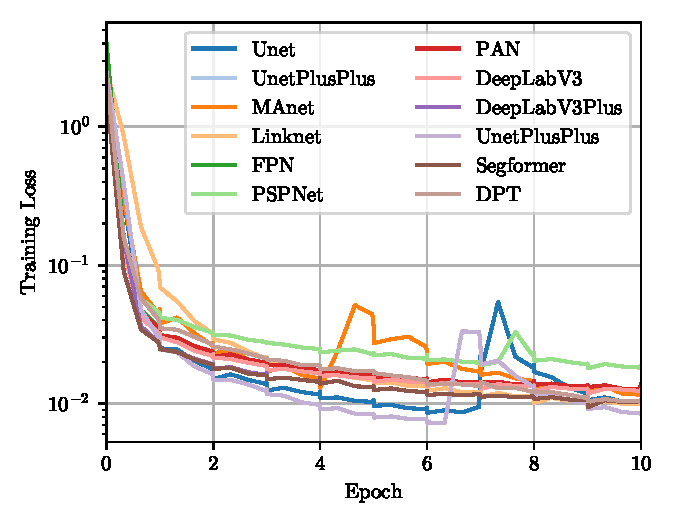
\includegraphics[width=\linewidth]{seg_2d/figures/LuSNAR_losses.pdf}
		\caption{\bfseries Training losses.}
		\label{fig:lusnar_losses}
	\end{subfigure}
	\begin{subfigure}[b]{\linewidth}
		\includegraphics[width=\linewidth]{seg_2d/figures/LuSNAR_losses_val.pdf}
		\caption{\bfseries Validation losses.}
		\label{fig:lusnar_val_losses}
	\end{subfigure}
	\caption{\bfseries Training and validation losses for the considered semantic segmentation models.}
\end{figure}
\begin{figure}[h!]
	\centering
	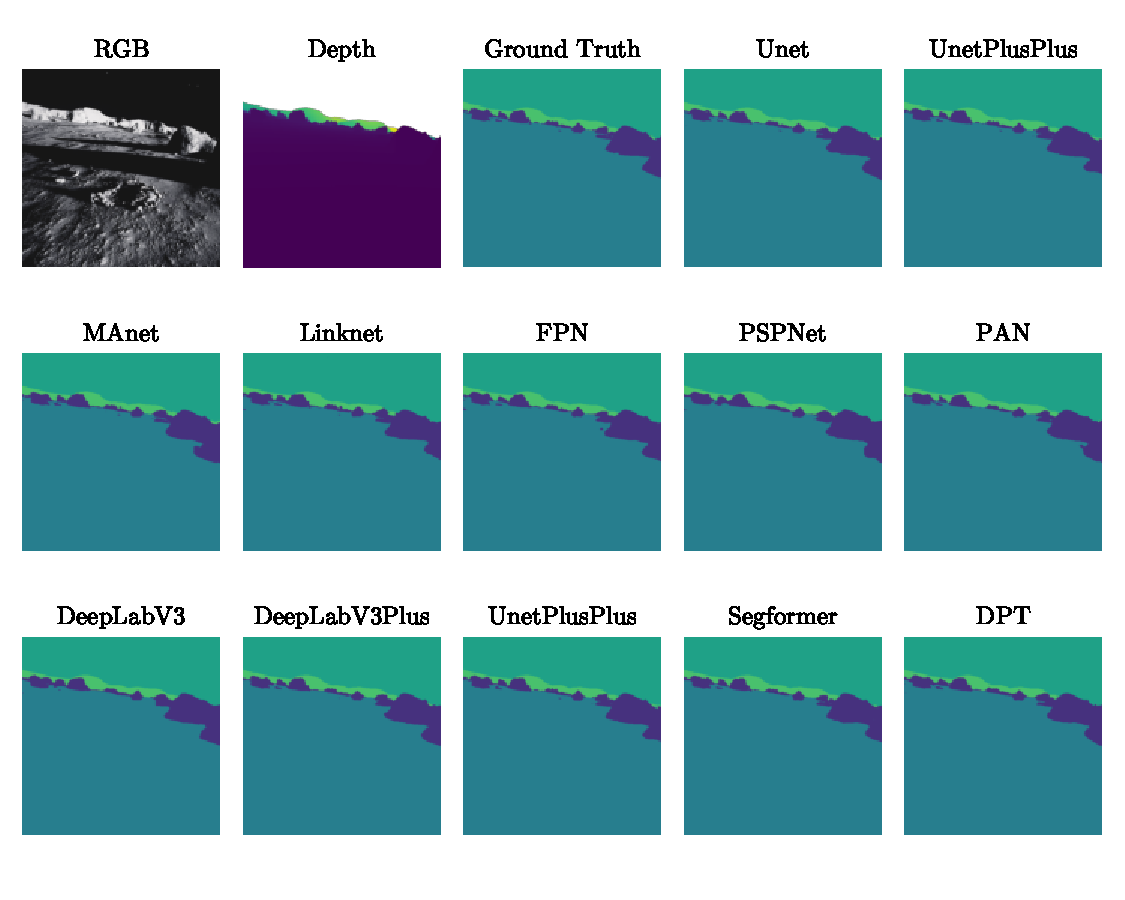
\includegraphics[width=\linewidth, trim={0 0em 0 0em}, clip]{seg_2d/figures/LuSNAR_predictions.pdf}
	\caption{\bfseries Test sample of semantic segmentation predictions for the LuSNAR dataset. Misclassied pixels are highlighted in red.}
	\label{fig:lusnar_predictions}
\end{figure}

\begin{table*}[h!]
	\centering
	\caption{\bfseries Semantic segmentation results on the LuSNAR dataset.}
	\label{tab:semantic_segmentation_models}
	\small
	\begin{tabular}{|l rrrrrrrrrr|}
		\hline
		\multicolumn{1}{|c}{\multirow{2}{*}{\textbf{Model}}}         &
		\multicolumn{1}{c}{\multirow{2}{*}{\textbf{Size [MB]}}}      &
		\multicolumn{1}{c}{\multirow{2}{*}{\textbf{Params}}}         &
		\multicolumn{1}{c}{\multirow{2}{*}{\textbf{FPS $\uparrow$}}} &
		\multicolumn{5}{c}{\textbf{IoU [\%] $\uparrow$}}             &
		\multicolumn{1}{c}{\textbf{Mean}}                            &
		\multicolumn{1}{c|}{\textbf{Mean}}
		\\
		\cmidrule{4-7}
		                                                             &               &               &               &
		\textbf{Regolith}                                            &
		\textbf{Crater}                                              &
		\textbf{Rock}                                                &
		\textbf{Mountain}                                            &
		\textbf{Sky}                                                 &
		\multicolumn{1}{c}{\textbf{IoU $\uparrow$}}                  &
		\multicolumn{1}{c|}{\textbf{Accuracy $\uparrow$}}
		\\
		\hline
		\hline
		U-Net                                                        & 55.0          & 14.3M         &
		114.4                                                        & \textbf{99.5} & 95.5          & 89.2          & 96.5          & \textbf{99.8} & 96.1          & 99.5          \\
		U-Net++                                                      & 61.0          & 16.0M         &
		78.0                                                         & \textbf{99.5} & 91.1          & \textbf{91.6} & \textbf{98.5} & \textbf{99.8} & 96.1          & \textbf{99.6} \\
		MA-Net                                                       & 83.0          & 21.7M         &
		71.7                                                         & 99.2          & 70.9          & 90.1          & 97.5          & \textbf{99.8} & 91.5          & 99.3          \\
		Linknet                                                      & 44.0          & 11.7M         &
		104.5                                                        & 99.2          & 96.4          & 91.1          & 97.0          & \textbf{99.8} & \textbf{96.7} & 99.3          \\
		FPN                                                          & 50.0          & 13.0M         &
		108.7                                                        & 98.9          & \textbf{97.7} & 86.8          & 97.8          & 99.7          & 96.2          & 99.2          \\
		PSPNet                                                       & \textbf{3.0}  & \textbf{0.9M} &
		\textbf{203.2}                                               & 98.8          & 92.7          & 79.7          & 94.3          & 99.6          & 93.0          & 99.0          \\
		PAN                                                          & 43.0          & 11.4M         &
		92.8                                                         & 99.0          & 94.6          & 84.3          & 97.4          & 99.7          & 95.0          & 99.2          \\
		DeepLabV3                                                    & 61.0          & 15.9M         &
		131.5                                                        & 99.0          & 96.7          & 86.6          & 98.3          & 99.7          & 96.1          & 99.2          \\
		DeepLabV3Plus                                                & 47.0          & 12.3M         &
		118.8                                                        & 99.2          & 96.4          & 89.2          & 98.0          & \textbf{99.8} & 96.5          & 99.4          \\
		Segformer                                                    & 45.0          & 11.8M         &
		140.5                                                        & 99.2          & 95.5          & 88.9          & 97.7          & \textbf{99.8} & 96.2          & 99.4          \\
		DPT                                                          & 159.0         & 41.6M         &
		79.6                                                         & 99.1          & 94.1          & 87.4          & 95.7          & 99.7          & 95.2          & 99.3          \\
		\hline
	\end{tabular}
\end{table*}

\subsection{Semantic Segmentation}
We benchmarked a suite of semantic segmentation architectures on the LuSNAR dataset to evaluate their effectiveness for lunar terrain classification. All models were trained to classify five semantic categories present in the dataset: regolith, craters, rocks, mountains, and sky~\cite{liu_lusnarlunar_2024}. The dataset was split into approximately 8,000 images for training, 1,000 for validation, and 2,000 for testing. For training, we used the Adam optimizer over 10 epochs with a batch size of 24. The initial learning rate was $1\times10^{-3}$, which was adjusted by a scheduler that reduced the rate by a factor of 0.75 with a patience of 10 epochs, down to a minimum of $1\times10^{-7}$.

As shown by the training and validation loss curves in \Cref{fig:lusnar_losses,fig:lusnar_val_losses}, all models converged successfully. Qualitatively, the majority of architectures are able to accurately segment the primary terrain features, with representative examples shown in \Cref{fig:lusnar_predictions}. The quantitative results in \Cref{tab:semantic_segmentation_models} reveal key performance trade-offs. While models like LinkNet and DeepLabV3+ achieve high overall mean IoU, other models excel at specific classes critical for navigation; for instance, FPN is the most effective at crater detection. Notably, PSPNet offers a highly efficient solution, achieving the highest FPS with by far the smallest model size, making it a strong candidate for resource-constrained hardware.
For our downstream mapping task, we selected U-Net++ due to having the best overall accuracy and IoU for rocks (91.6\% IoU), a critical capability for ensuring rover safety, while being computationally comparable to the other models.

% \begin{figure}[h]
%     \centering
%     \begin{subfigure}[b]{\linewidth}
%         \centering
%         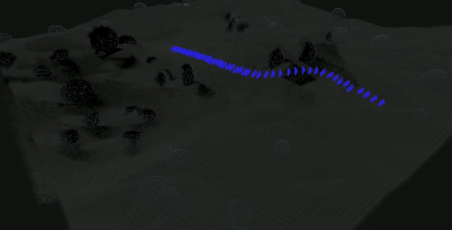
\includegraphics[width=0.8\textwidth]{gaussians_1.png}
%         \caption{\bfseries Ground truth depth and segmentation.}
%         \label{fig:gaussians_1}
%     \end{subfigure}
%     \begin{subfigure}[b]{\linewidth}
%         \centering
%         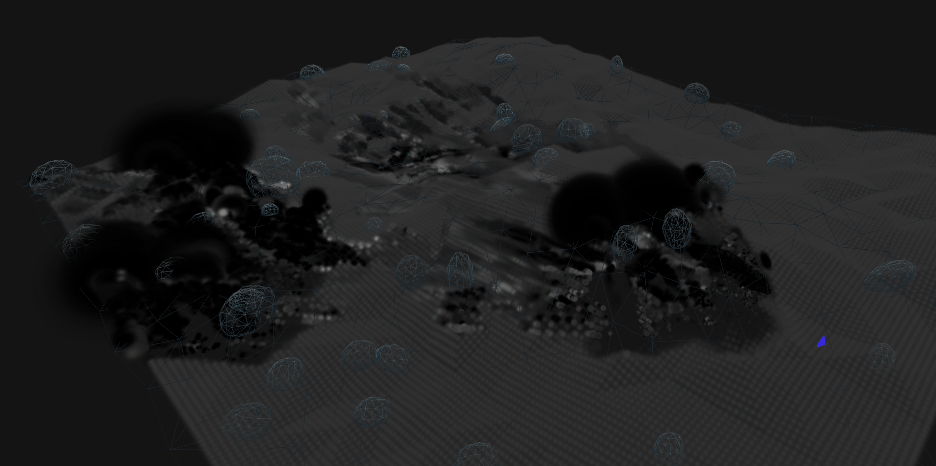
\includegraphics[width=0.8\textwidth]{gaussians_3.png}
%         \caption{\bfseries RAFT-Stereo depth and U-Net++ segmentation.}
%         \label{fig:gaussians_3}
%     \end{subfigure}
%     \caption{\bfseries Effect of depth estimation and segmentation on 3D Gaussian Splatting.}
% \end{figure}
